\documentclass[serif]{beamer}\usepackage[]{graphicx}\usepackage[]{color}
%% maxwidth is the original width if it is less than linewidth
%% otherwise use linewidth (to make sure the graphics do not exceed the margin)
\makeatletter
\def\maxwidth{ %
  \ifdim\Gin@nat@width>\linewidth
    \linewidth
  \else
    \Gin@nat@width
  \fi
}
\makeatother

\definecolor{fgcolor}{rgb}{0.345, 0.345, 0.345}
\newcommand{\hlnum}[1]{\textcolor[rgb]{0.686,0.059,0.569}{#1}}%
\newcommand{\hlstr}[1]{\textcolor[rgb]{0.192,0.494,0.8}{#1}}%
\newcommand{\hlcom}[1]{\textcolor[rgb]{0.678,0.584,0.686}{\textit{#1}}}%
\newcommand{\hlopt}[1]{\textcolor[rgb]{0,0,0}{#1}}%
\newcommand{\hlstd}[1]{\textcolor[rgb]{0.345,0.345,0.345}{#1}}%
\newcommand{\hlkwa}[1]{\textcolor[rgb]{0.161,0.373,0.58}{\textbf{#1}}}%
\newcommand{\hlkwb}[1]{\textcolor[rgb]{0.69,0.353,0.396}{#1}}%
\newcommand{\hlkwc}[1]{\textcolor[rgb]{0.333,0.667,0.333}{#1}}%
\newcommand{\hlkwd}[1]{\textcolor[rgb]{0.737,0.353,0.396}{\textbf{#1}}}%
\let\hlipl\hlkwb

\usepackage{framed}
\makeatletter
\newenvironment{kframe}{%
 \def\at@end@of@kframe{}%
 \ifinner\ifhmode%
  \def\at@end@of@kframe{\end{minipage}}%
  \begin{minipage}{\columnwidth}%
 \fi\fi%
 \def\FrameCommand##1{\hskip\@totalleftmargin \hskip-\fboxsep
 \colorbox{shadecolor}{##1}\hskip-\fboxsep
     % There is no \\@totalrightmargin, so:
     \hskip-\linewidth \hskip-\@totalleftmargin \hskip\columnwidth}%
 \MakeFramed {\advance\hsize-\width
   \@totalleftmargin\z@ \linewidth\hsize
   \@setminipage}}%
 {\par\unskip\endMakeFramed%
 \at@end@of@kframe}
\makeatother

\definecolor{shadecolor}{rgb}{.97, .97, .97}
\definecolor{messagecolor}{rgb}{0, 0, 0}
\definecolor{warningcolor}{rgb}{1, 0, 1}
\definecolor{errorcolor}{rgb}{1, 0, 0}
\newenvironment{knitrout}{}{} % an empty environment to be redefined in TeX

\usepackage{alltt}
\usetheme{Boadilla}
\usepackage{graphicx}
\usepackage[draft]{animate}
\usepackage{breqn}
\usepackage{xcolor}
\usepackage{booktabs}
\usepackage{tikz}
\usetikzlibrary{decorations.pathreplacing}
\usetikzlibrary{shapes,arrows,positioning,shadows}
\usepackage{subfig}
\usepackage{pgf}

% change format of enumerated lists
\setbeamertemplate{enumerate items}[default]

\setbeamertemplate{navigation symbols}{}

% custom colors
\definecolor{mypal1}{HTML}{F0F9E8}\definecolor{mypal2}{HTML}{BAE4BC}\definecolor{mypal3}{HTML}{7BCCC4}\definecolor{mypal4}{HTML}{43A2CA}\definecolor{mypal5}{HTML}{0868AC}

\tikzstyle{decision} = [diamond, draw, text width=6em, text badly centered, inner sep = 2pt, top color=white, bottom color=mypal3, drop shadow]
\tikzstyle{block} = [rectangle, draw, text width=10em, text centered, rounded corners, minimum height=3em, minimum width=8em, top color = white, bottom color=mypal4,  drop shadow]
\tikzstyle{declare} = [rectangle, draw, text width=10em, text centered, minimum height=3em, minimum width=8em, top color = white, bottom color=mypal5,  drop shadow]

% knitr setup


% dependent data


% get online bib file


% my custom ggplot theme


\setbeamercolor{title}{fg=mypal5} % main title
\setbeamercolor{frametitle}{fg=mypal4, bg=mypal2} % frame titles
\setbeamercolor{structure}{fg=mypal4} % bottom banner
\setbeamercolor{normal text}{fg=mypal5}
\usebackgroundtemplate{
\includegraphics[height=\paperheight,width=\paperwidth]{fig/back_tmp.pdf}}

% macros
\newcommand{\emtxt}[1]{\textbf{\textit{#1}}}
\IfFileExists{upquote.sty}{\usepackage{upquote}}{}
\begin{document}

\title[Memoirs of a GED post-doc]{\textbf{Nutrients, estuaries, and coffee: Memoirs of a GED post-doc}}
\author[M. Beck]{Marcus W. Beck, Ph.D.}

\institute[USEPA]{USEPA National Health and Environmental Effects Research Laboratory, Gulf Ecology Division, \href{mailto:beck.marcus@epa.gov}{beck.marcus@epa.gov}, Phone: 8509342480}

\date{August 28, 2017}

\titlegraphic{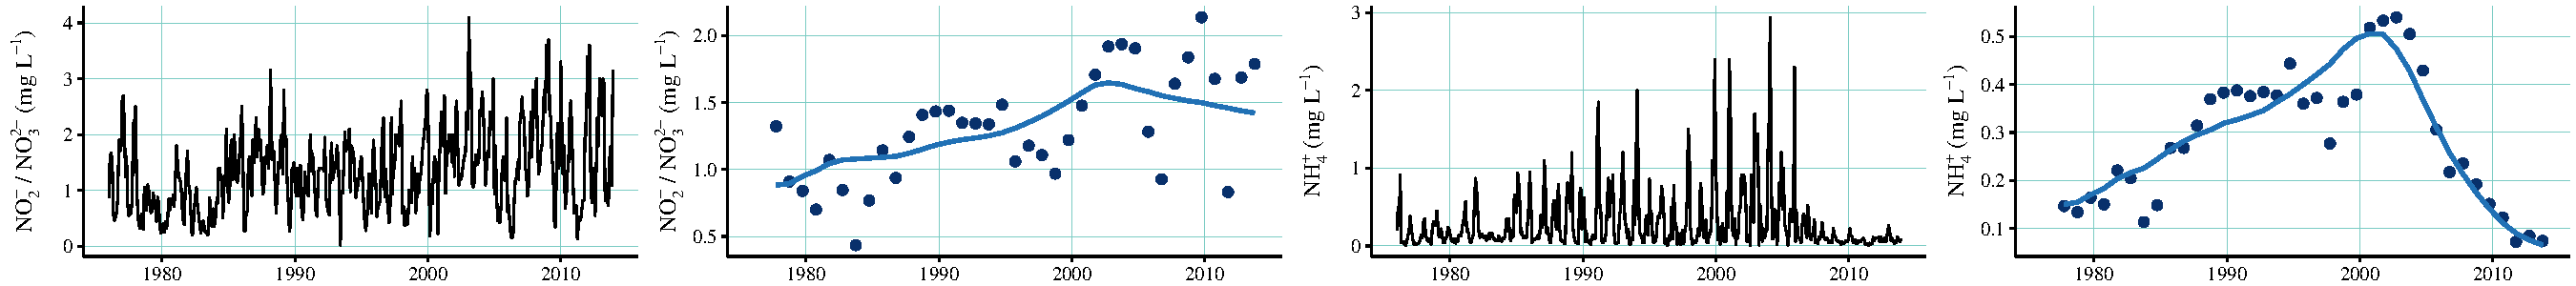
\includegraphics[trim = 0cm 0cm 0cm -3cm,clip=true,width=\linewidth]{fig/titlegraphic.pdf}}

%%%%%%
\begin{frame}[shrink]
\titlepage
\end{frame}

\section{Background}

%%%%%%
\begin{frame}{Why are we here today?}{}
\begin{columns}
\begin{column}{0.5\textwidth}
\begin{center}
\fbox{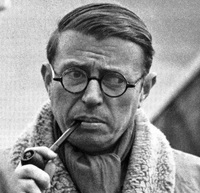
\includegraphics[width=0.8\textwidth]{fig/Sartre1.jpg}}
\end{center}
\end{column}
\begin{column}{0.5\textwidth}
\begin{quote}
\Large
Freedom is what you do with what's been done to you.\\~\\
\vspace{0.05in}
\hfill -- J. P. Sartre\\~\\
\end{quote}
\end{column}
\end{columns}
\end{frame}

%%%%%%
\begin{frame}{Why are we here today?}{}
\begin{columns}
\begin{column}{0.5\textwidth}
\onslide<+->
\begin{center}
\fbox{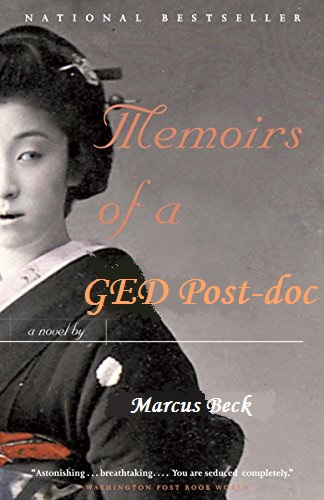
\includegraphics[width=0.6\textwidth]{fig/geisha.jpg}}
\end{center}
\end{column}
\begin{column}{0.5\textwidth}
\begin{itemize}
\item<+-> Where did I come from? \\~\\
\item<+-> The ORISE experience \\~\\
\item<+-> The EPA experience \\~\\
\item<+-> The next chapter \\~\\
\item<+-> Final thoughts/ramblings 
\end{itemize}
\end{column}
\end{columns}\end{frame}

\section{Where did I come from?}

%%%%%%
\begin{frame}{Where did I come from?}{}
Minnesota, the land of 11,842 lakes
\begin{columns}
\begin{column}{0.5\textwidth}
\centerline{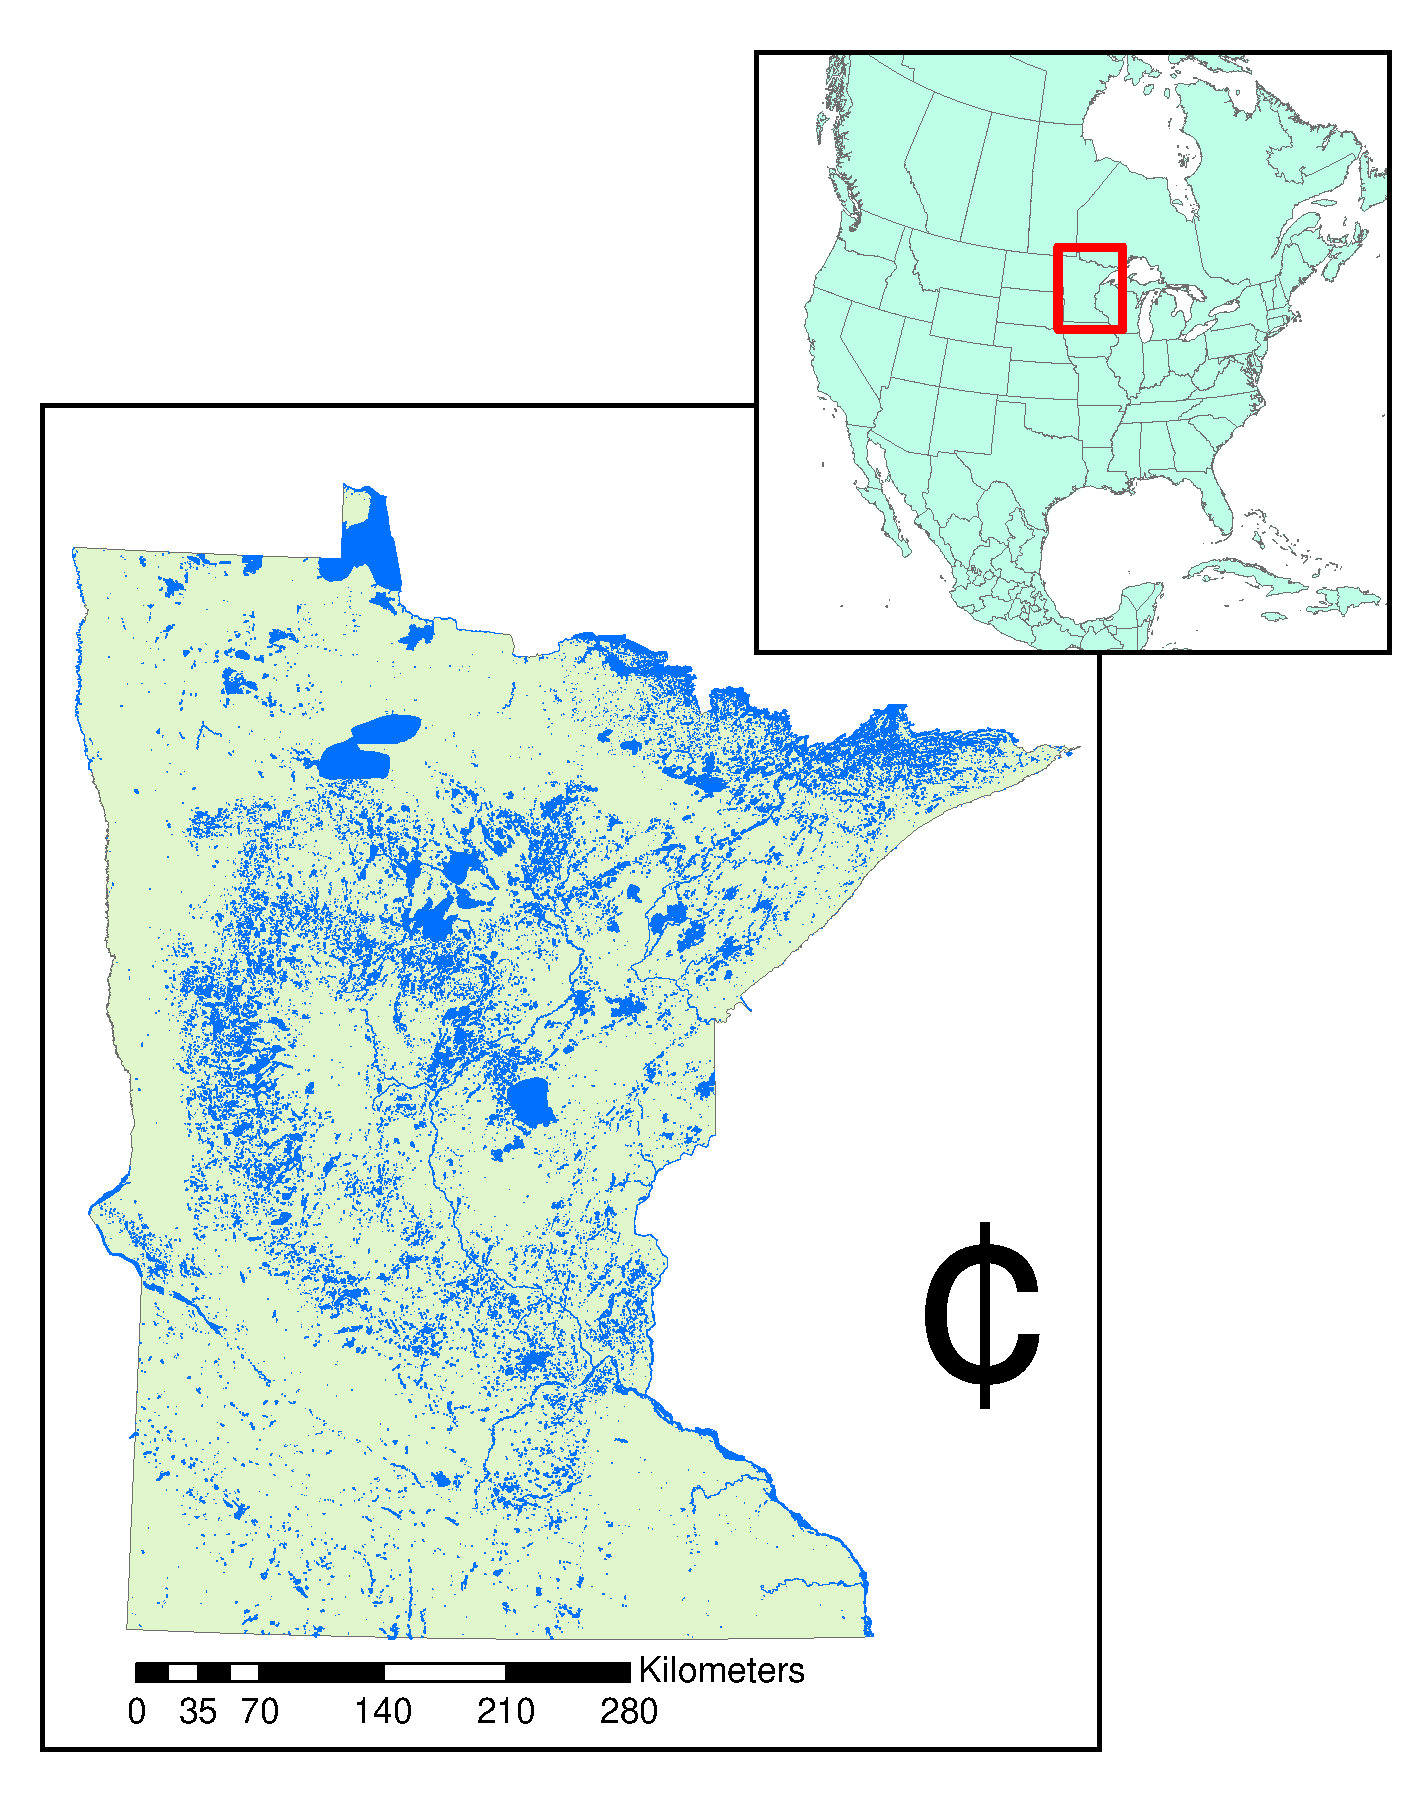
\includegraphics[width=\textwidth]{fig/mn_lake_inset.pdf}}
\end{column}
\begin{column}{0.5\textwidth}
\begin{center}

\includegraphics[width=0.5\textwidth]{fig/mn_seal.jpg} \\~\\
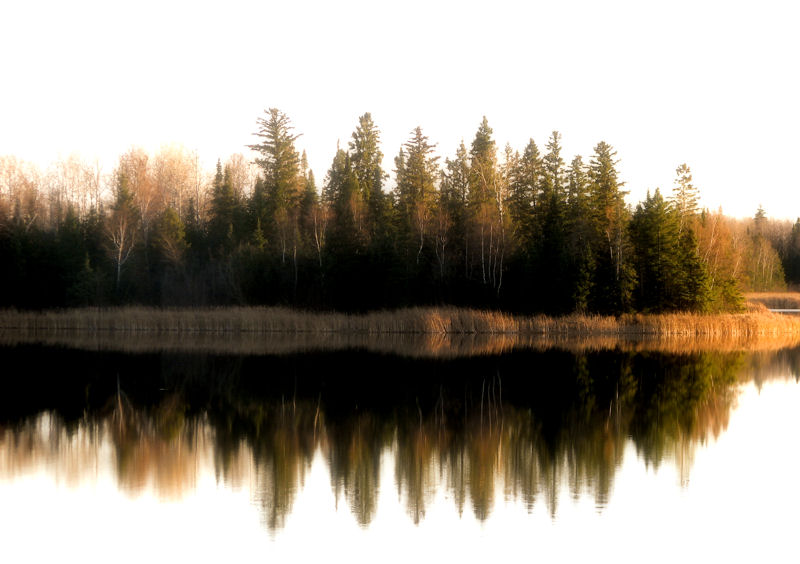
\includegraphics[width=0.8\textwidth]{fig/mn_lake.jpg}
\end{center}
\end{column}
\end{columns}
\end{frame}

%%%%%%
\begin{frame}{Where did I come from?}{}
\begin{itemize}
\item Dataset of 332 vegetation surveys, courtesy of MNDNR \cite{Beck14a}
\item Environmental data describing lake characteristics and anthropogenic stressors
\end{itemize}
\begin{columns}
\begin{column}{0.5\textwidth}
\centerline{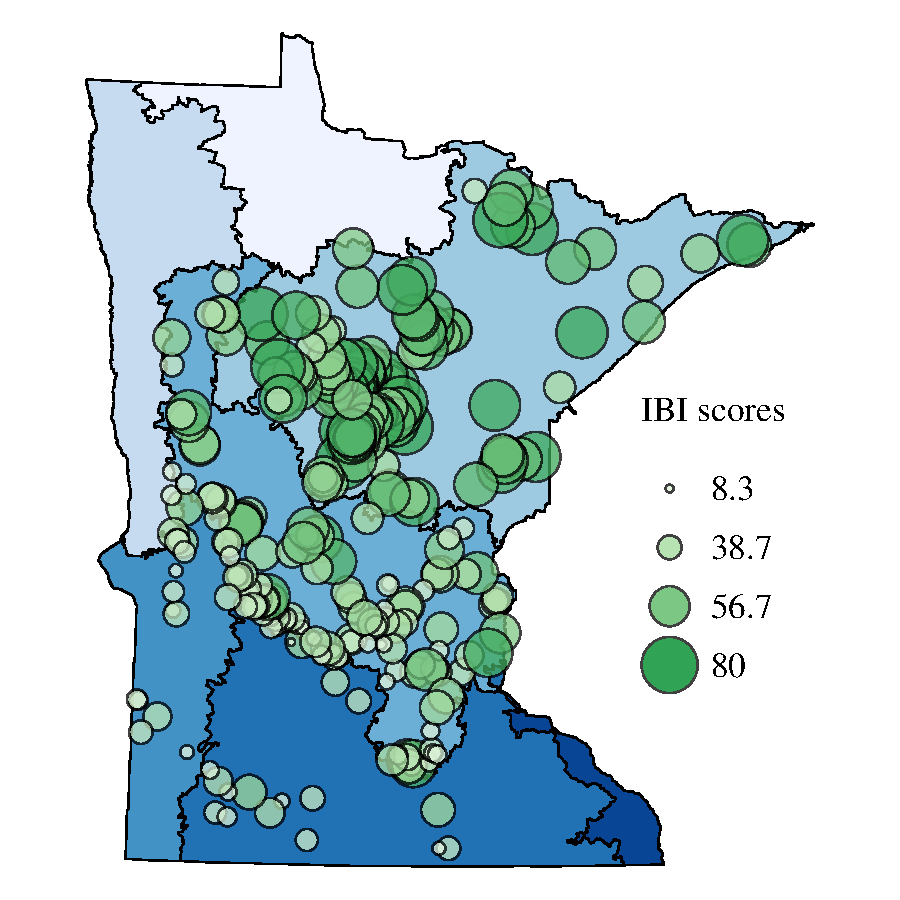
\includegraphics[width=0.9\textwidth]{fig/Beck_GEDsem-ibi_data.pdf}}
\end{column}
\begin{column}{0.5\textwidth}
\scriptsize
\begin{itemize}
\item{lake surface area}
\item{maximum lake depth}
\item{trophic state index}
\item{growing degree days}
\item{percent agriculture in wshed}
\item{percent impervious surfaces in wshed}
\item{density of groundwater wells in wshed}
\item{wshed area to lake area}
\item{crop productivity index of wshed}
\item{dock density}
\item{...}
\end{itemize}
\end{column}
\end{columns}
\end{frame}

\section{The ORISE experience}

%%%%%%
\begin{frame}{The ORISE experience}{}
\centerline{\emtxt{July 2013, moved to Pensacola}}
\vspace{0.15in}
\centerline{\fbox{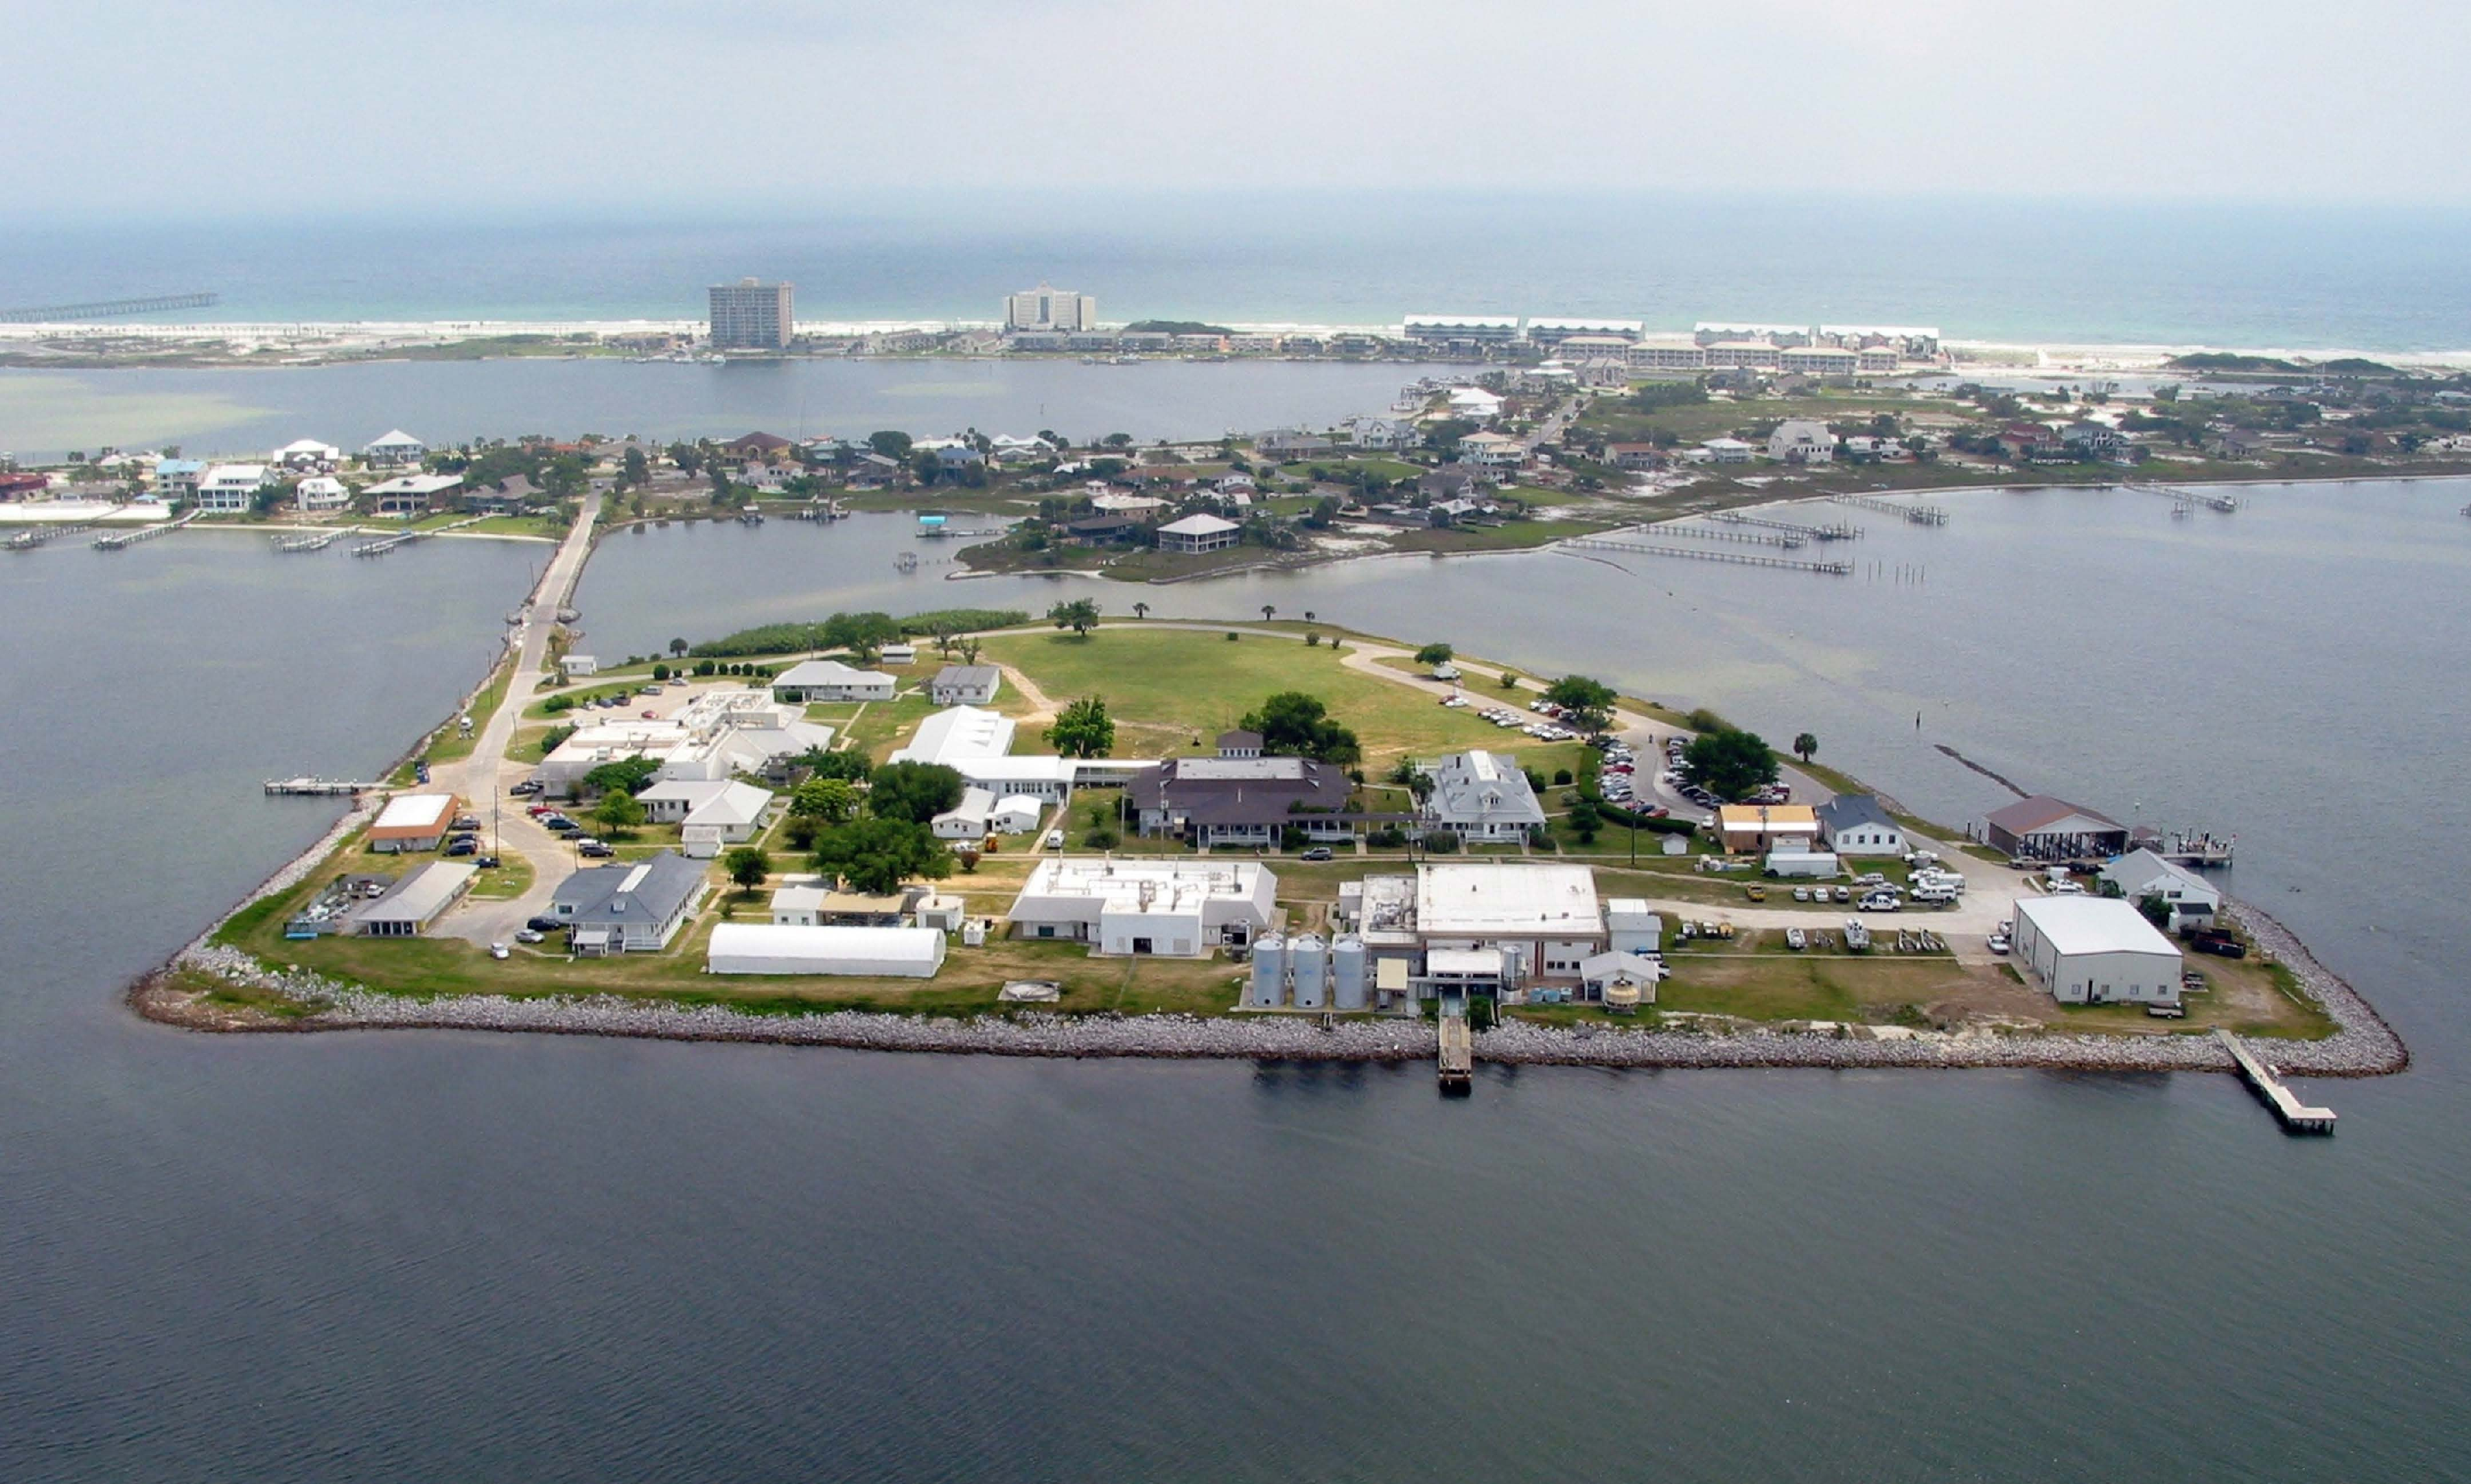
\includegraphics[width = 0.8\textwidth]{fig/sabine.pdf}}}
\end{frame}

%%%%%%
\begin{frame}{The ORISE experience}{}
\begin{columns}
\begin{column}{0.67\textwidth}

\includegraphics[width=\textwidth]{fig/orise.jpg}
\end{column}
\begin{column}{0.33\textwidth}

\includegraphics[width=\textwidth]{fig/orau.jpg}
\end{column}
\end{columns}
\vspace{0.2in}
\begin{itemize}
\item<+-> ORISE is a mysterious entity \\~\\
\item<+-> You are not an EPA employee \\~\\
\item<+-> EPA employees cannot tell you what to do \\~\\
\item<+-> You are not responsible for anything
\end{itemize}
\end{frame}

%%%%%%
\begin{frame}{The ORISE experience}{Tampa Bay trend analysis}
\begin{columns}
\begin{column}{0.5\textwidth}
\begin{itemize}
\item Four bay segments\\~\\
\item Monthly wq data at 50 stations from 1974 to present \\~\\
\item Longitudinal profile of nutrient load and salinity \\~\\
\end{itemize}
\vspace{0cm}\hspace*{15pt}\scalebox{0.7}{\hbox{\tiny Data from \cite{TBEP11}}}
\end{column}
\begin{column}{0.5\textwidth}
\centerline{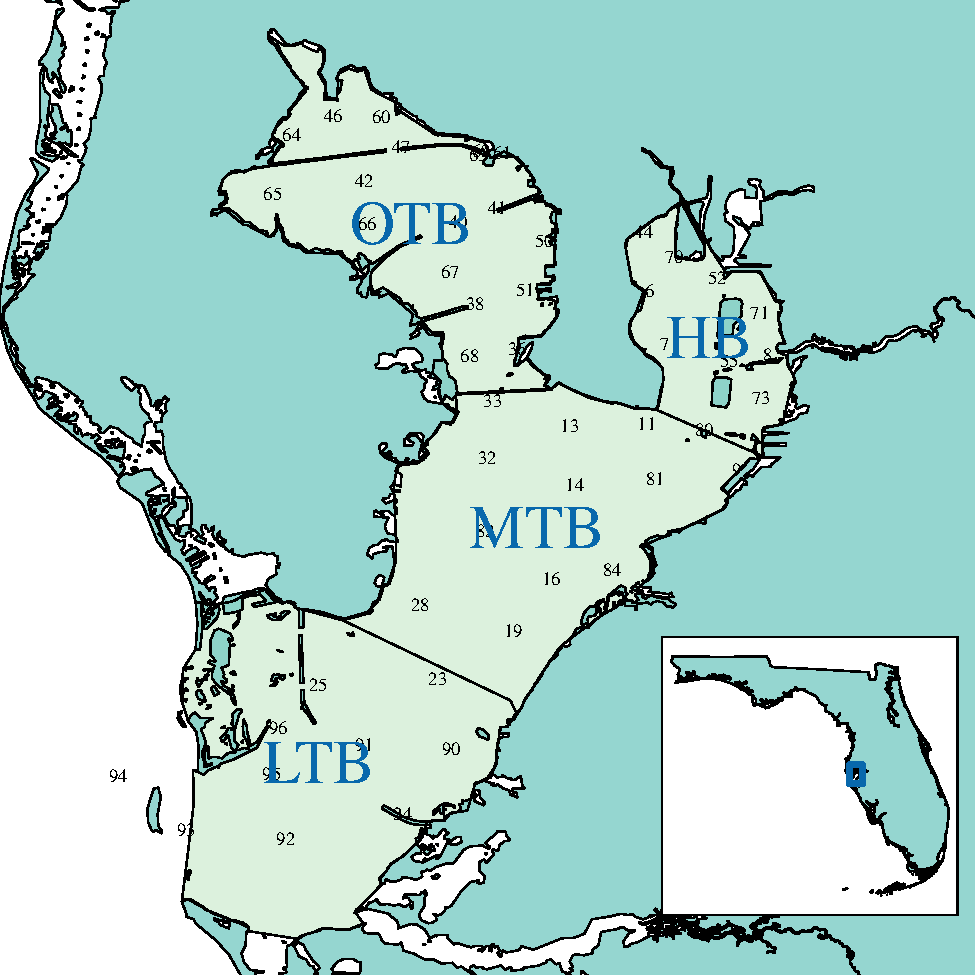
\includegraphics[width = \textwidth]{fig/tb_map.pdf}}
\end{column}
\end{columns}
\end{frame}

%%%%%%
\begin{frame}{The ORISE experience}{Tampa Bay trend analysis}
\centerline{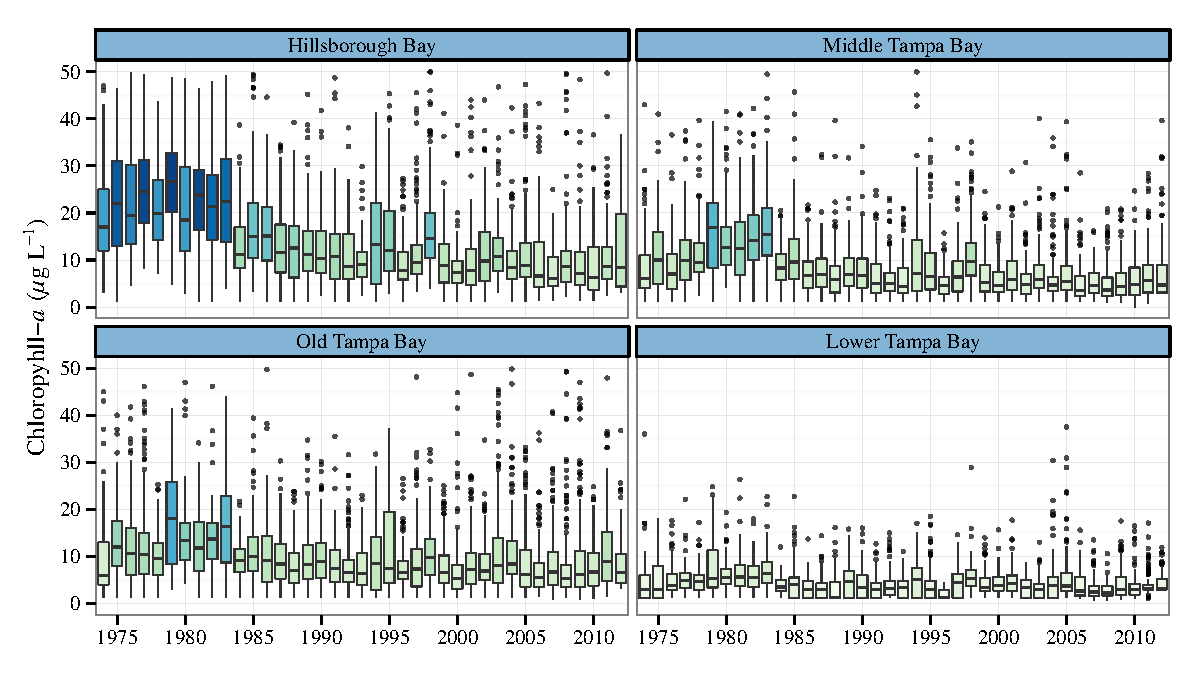
\includegraphics[width = \textwidth]{fig/annual_chl-1.pdf}}
\end{frame}

%%%%%%
\begin{frame}{The ORISE experience}{Tampa Bay trend analysis}
\onslide<+->
\begin{block}{Study objective}
Adapt and apply a nutrient response model for estuaries that leverages the descriptive capabilities of large datasets \scriptsize \cite{Beck15}
\end{block}
\vspace{0.2in}
\onslide<+->
Questions of concern -- Can we...
\begin{itemize}
\item ...provide a natural history of water quality that is temporally consistent with drivers of change?
\onslide<+->
\item ...improve our understanding of the nutrient-response paradigm in estuaries?
\end{itemize}
\end{frame}

%%%%%%
\begin{frame}[t]{The ORISE experience}{Tampa Bay trend analysis}
\onslide<1->
How does it work?  
\begin{center}
$\ln\left(N\right) = \beta_0 + \beta_1 t + \beta_2 Sal + \beta_3 \sin\left(2\pi t\right) + \beta_4 \cos\left(2\pi t\right)$\\~\\
$N$: nitrogen (or other response endpoint)\\
$t$: time\\
$Sal$: Salinity (or other flow-related variable)
\end{center}
\includegraphics<2>[width = \textwidth, page = 1]{fig/wrtds_pieces.pdf}
\includegraphics<3>[width = \textwidth, page = 2]{fig/wrtds_pieces.pdf}
\includegraphics<4>[width = \textwidth, page = 3]{fig/wrtds_pieces.pdf}
\includegraphics<5>[width = \textwidth, page = 4]{fig/wrtds_pieces.pdf}
\includegraphics<6>[width = \textwidth, page = 5]{fig/wrtds_pieces.pdf}
\end{frame}

%%%%%%
\begin{frame}{The ORISE experience}{Tampa Bay trend analysis}
{\small
\emtxt{Points}: observed time series (black are weighted, grey is zero weight)\\
\emtxt{Green point}: observation at the center of the regression\\
\emtxt{Blue line}: Global model with weights specific to the window\\
\emtxt{Red line}: Accumulated WRTDS model
}
\begin{center}
\animategraphics[controls,width=\linewidth]{10}{fig/wrtds_pieces2}{}{} %frame rate is 12 per/sec
\end{center}
\end{frame}

%%%%%%
\begin{frame}{The ORISE experience}{Tampa Bay trend analysis}
\centerline{RMSE fit for unweighted = 0.58, WRTDS = 0.36}
\begin{center}
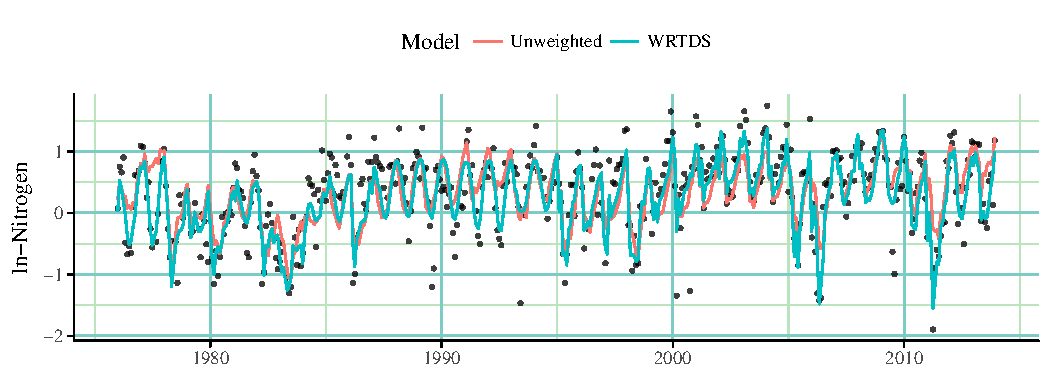
\includegraphics[width = \textwidth]{fig/wrtds_perf.pdf}
\end{center}
\end{frame}

%%%%%%
\begin{frame}{The ORISE experience}{Tampa Bay trend analysis}
Because the model is dynamic, we have parameters describing the relationship of chlorophyll with other factors specific to different time periods \\~\\
\begin{columns}[T]
\begin{column}{0.45\textwidth}
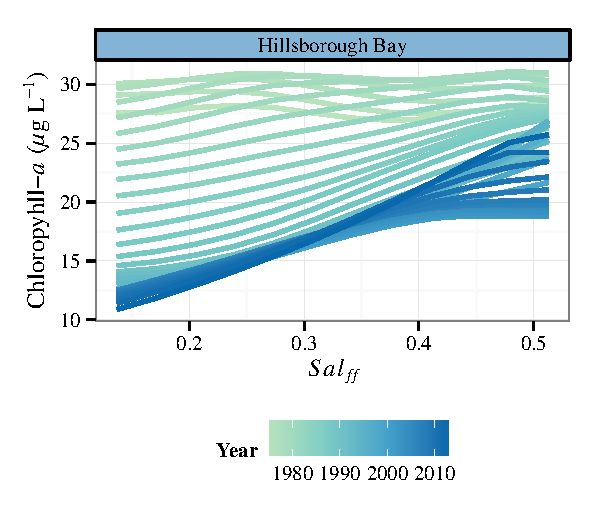
\includegraphics[width = \textwidth]{fig/hill-1.pdf}
\end{column}
\begin{column}{0.45\textwidth}
\begin{itemize}
\item Early period (light blue) - point-sources
\item Late period (dark blue) - non-point sources
\item Chlorophyll shows increasing response to freshwater input in recent years
\end{itemize}
\end{column}
\end{columns}
\end{frame}

%%%%%%
\begin{frame}{The ORISE experience}{Tampa Bay trend analysis}
\onslide<+->
\begin{figure}
\centerline{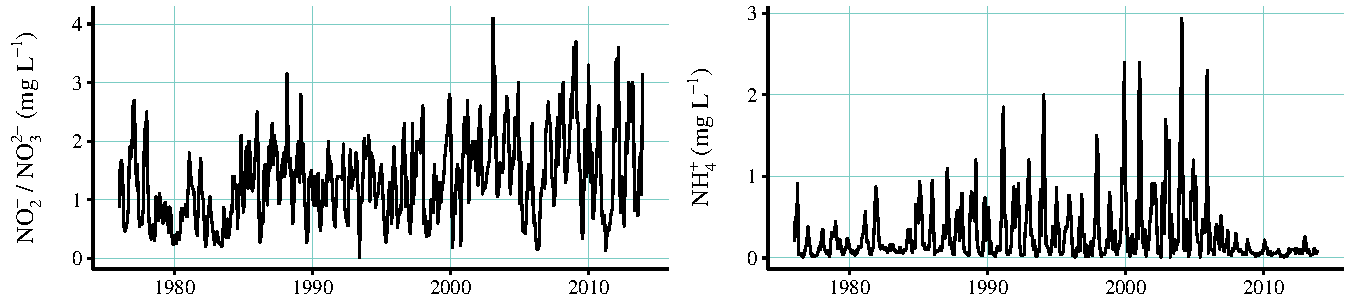
\includegraphics[width = \textwidth]{fig/p8obs.pdf}}
\caption{Observed nitrogen time series at P8 (SF Bay Delta RMP)}
\end{figure}
\onslide<+->
\vspace{-0.35in}
\begin{figure}
\centerline{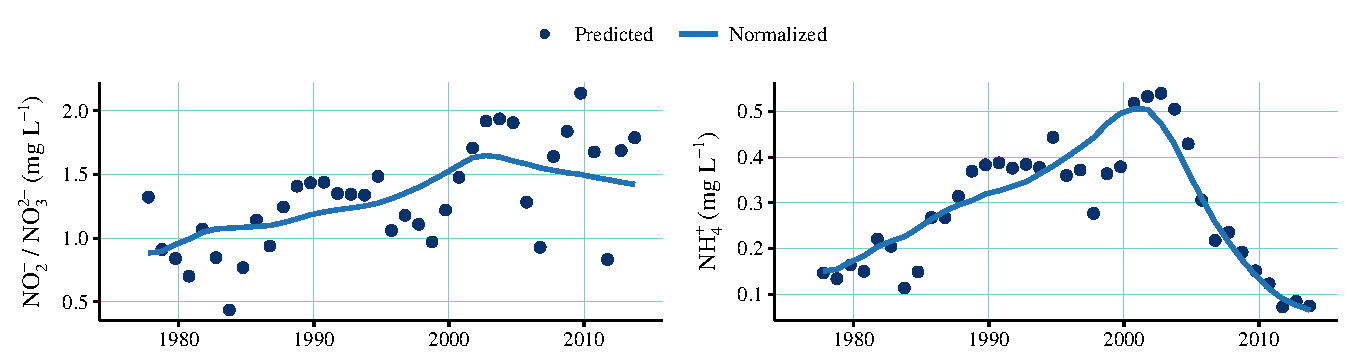
\includegraphics[width = \textwidth]{fig/p8prdnrm.pdf}}
\caption{Annual predicted and flow-normalized nitrogen from WRTDS.}
\end{figure}
\end{frame}

%%%%%%
\begin{frame}{The ORISE experience}{Time series detiding}
The `Odum' open-water method has been used for decades to estimate rates of ecosystem metabolism \scriptsize \cite{Odum56} \\~\\
\normalsize
\begin{center}
$\frac{\delta DO}{\delta t} = P - R + D$
\end{center}
Metabolic rates provide a measure of productivity in a system - are estuaries sources or sinks of organic matter? \scriptsize \cite{Caffrey14}
\normalsize \\~\\
Applications to estuarine monitoring data have been somewhat successful - why?? 
\end{frame}

%%%%%%
\begin{frame}{The ORISE experience}{Time series detiding}
The `Odum' method assumes DO represents biological processes...


{\centering 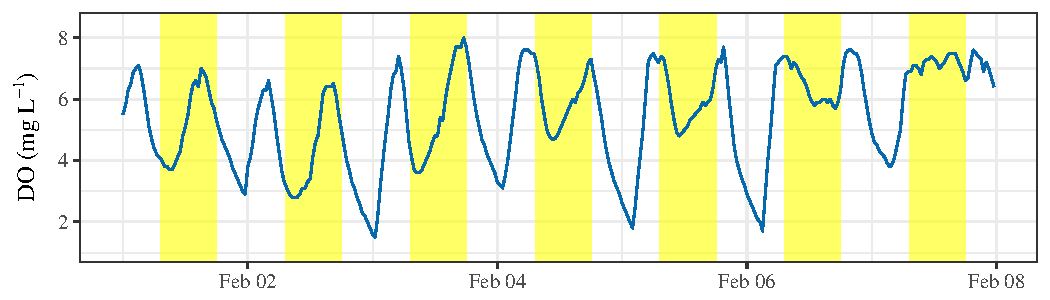
\includegraphics[width=0.95\textwidth]{fig/sapdo-1} 

}





{\centering 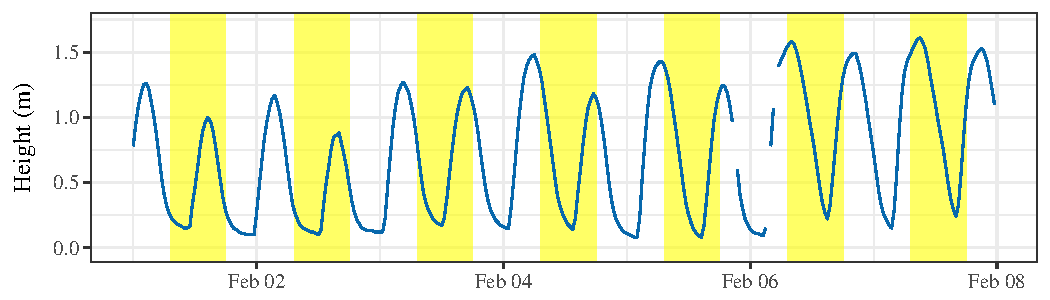
\includegraphics[width=0.95\textwidth]{fig/saptide-1} 

}



\end{frame}



%%%%%%
\begin{frame}{The ORISE experience}{Time series detiding}
\begin{center}
\animategraphics[controls,width=\linewidth]{25}{fig/detide_ani}{1}{169} %frame rate is 50 per/sec
\end{center}
\end{frame}

%%%%%%
\begin{frame}{The ORISE experience}{Time series detiding}
DO time series and ecosystem metabolism {\footnotesize\cite{Beck15b}}
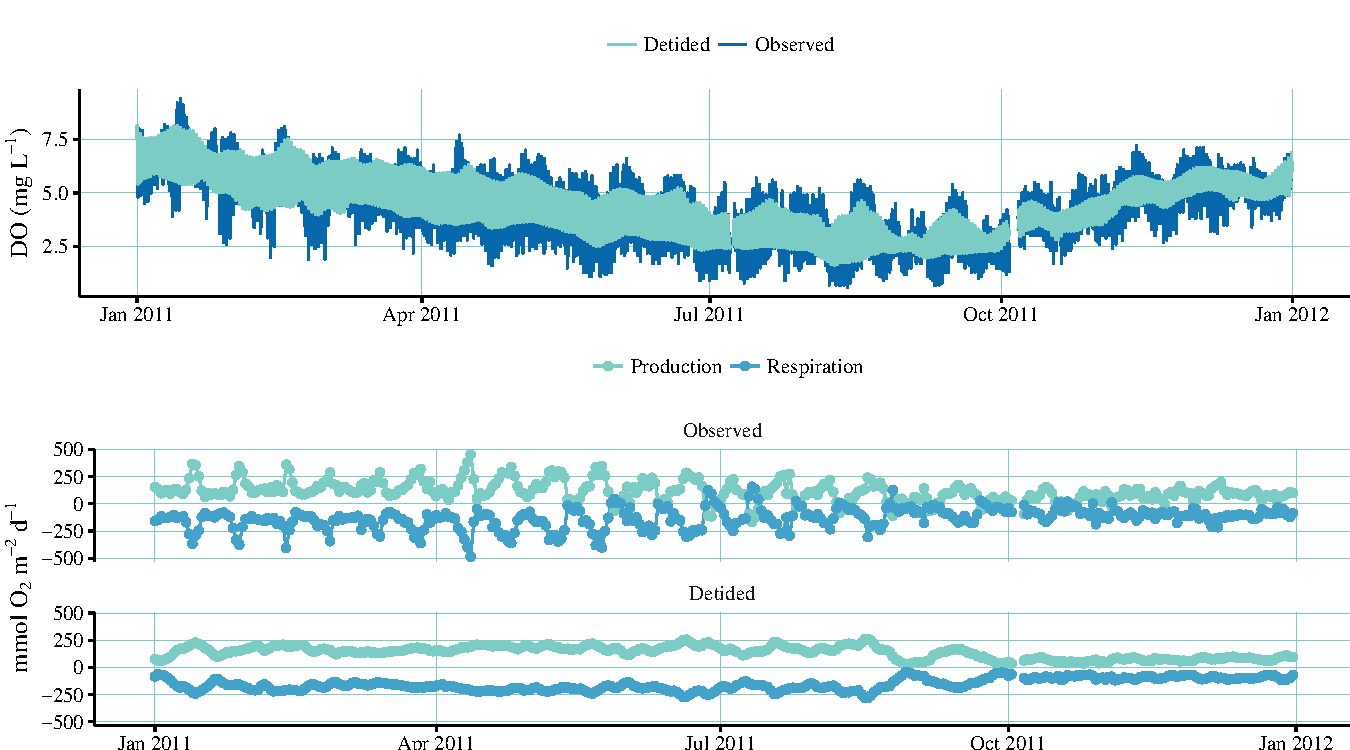
\includegraphics[width = \textwidth]{fig/metex.pdf}
\end{frame}

%%%%%%
\begin{frame}{The ORISE experience}{Additional WRTDS applications}
Comparing WRTDS and GAMs for trend evaluation {\footnotesize \cite{Beck17}}
\begin{columns}
\begin{column}{0.38\textwidth}
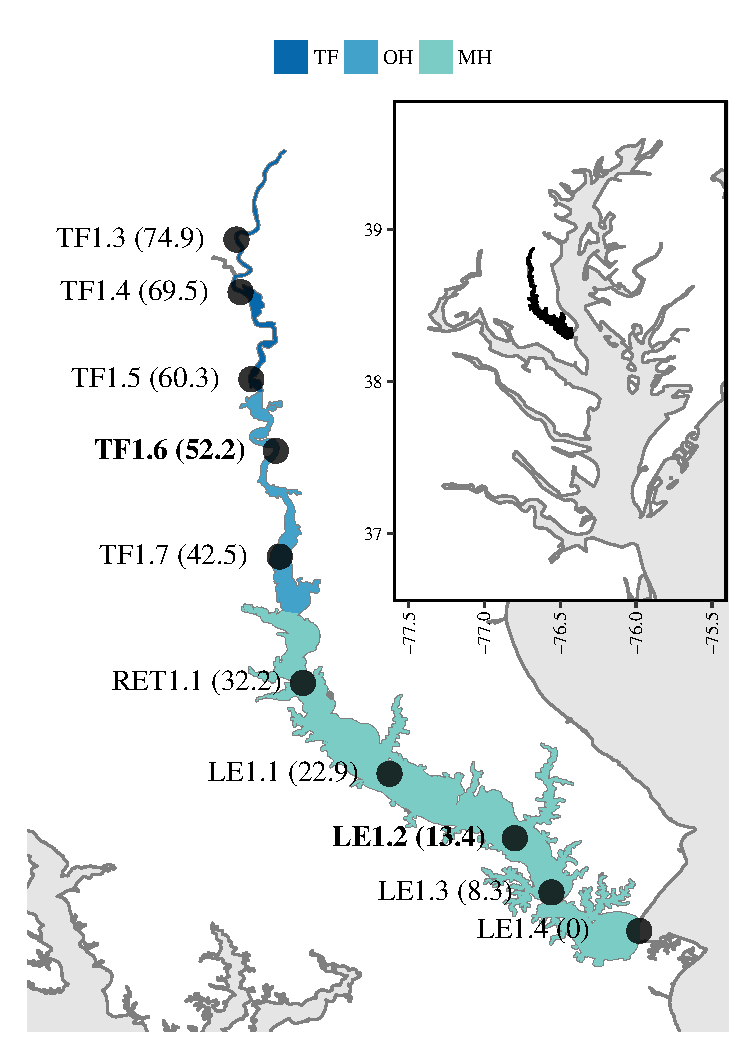
\includegraphics[width = \textwidth]{fig/patux_map.pdf}
\end{column}
\begin{column}{0.65\textwidth}
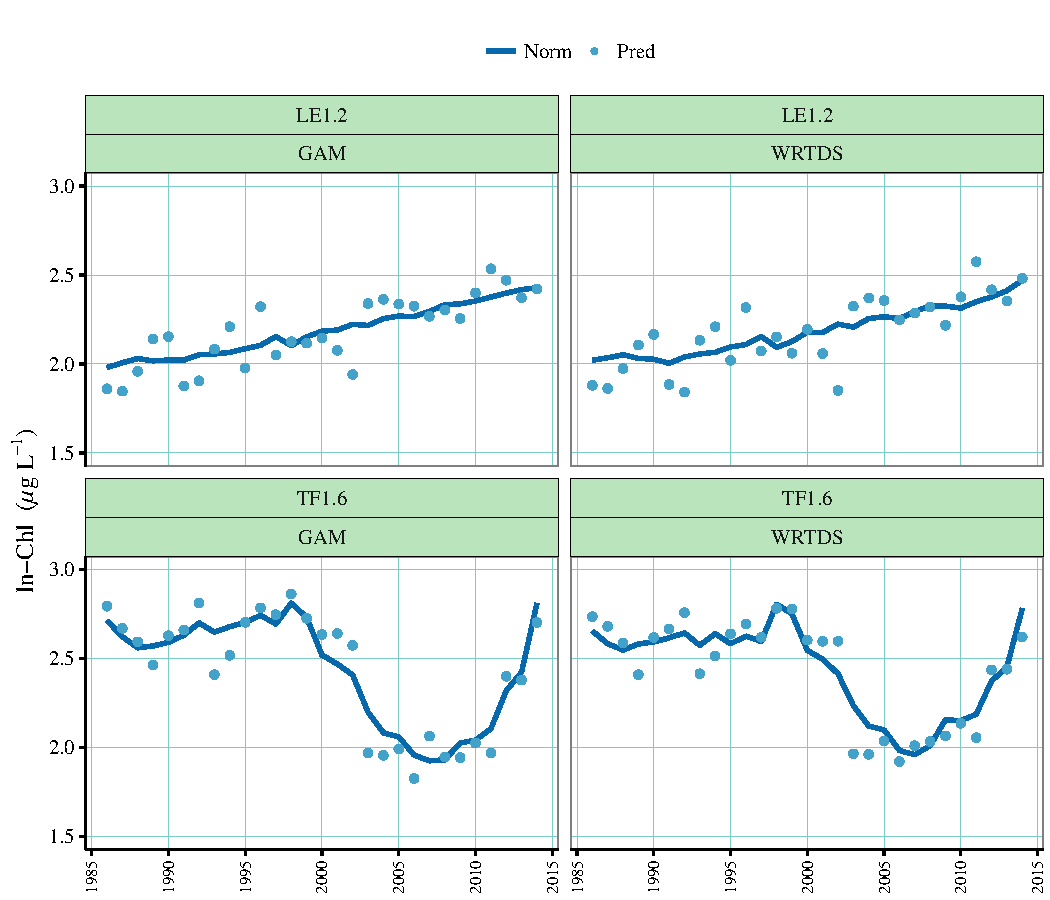
\includegraphics[width = \textwidth]{fig/predann.pdf}
\end{column}
\end{columns}
\end{frame}

%%%%%%
\begin{frame}{The ORISE experience}{Additional WRTDS applications}
\centerline{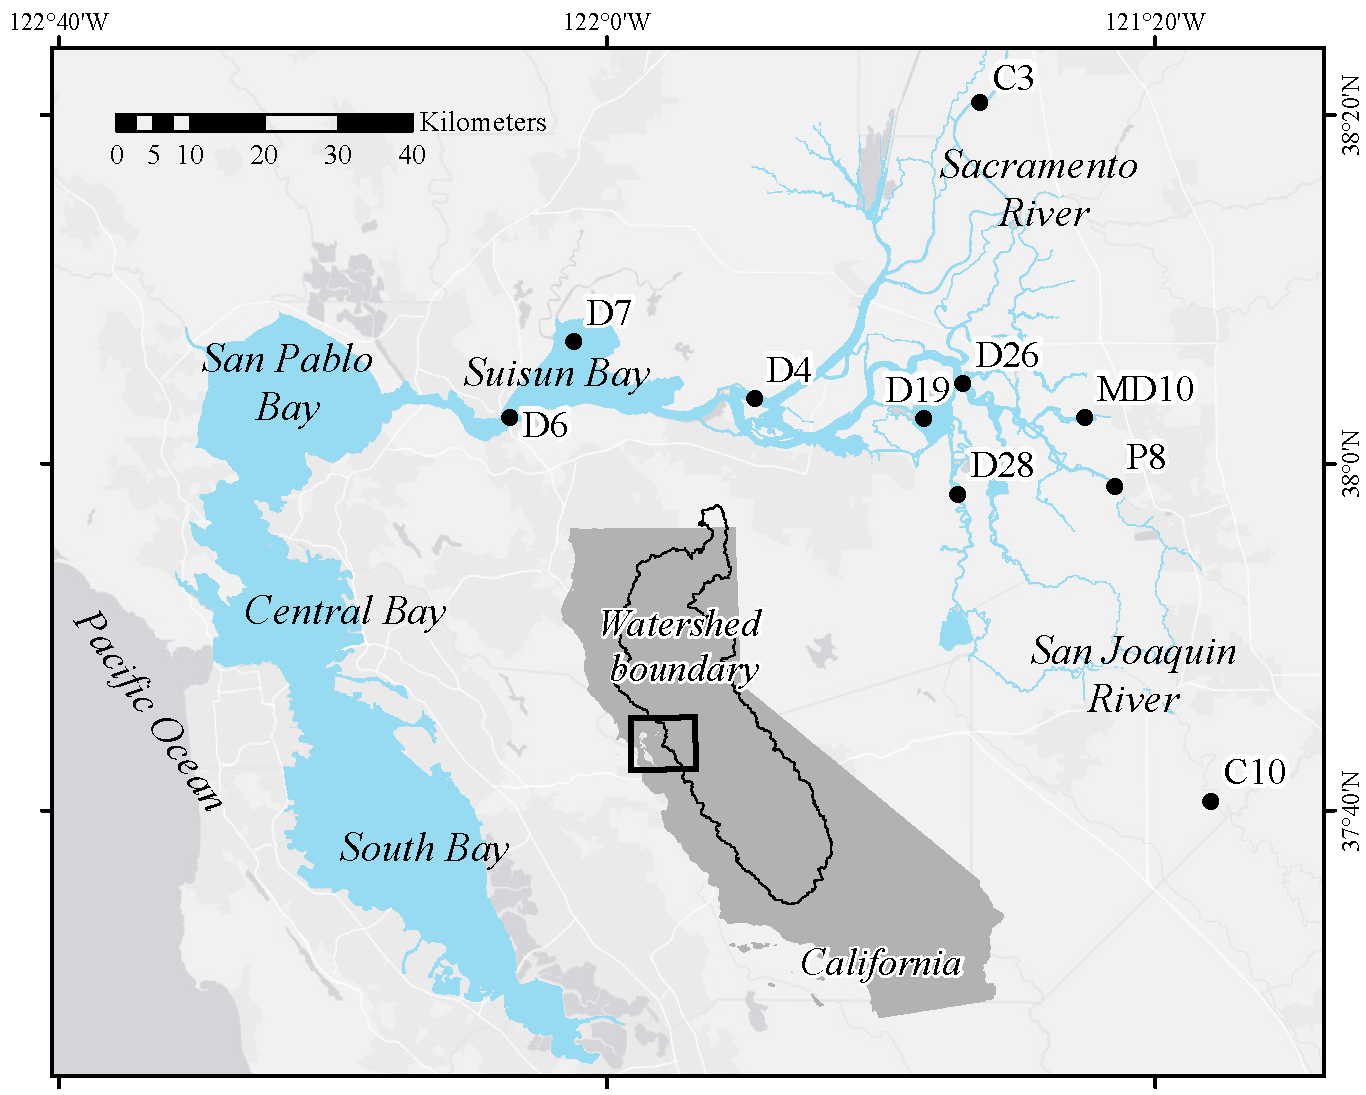
\includegraphics[width = 0.75\textwidth]{fig/delt_map.pdf}}
\end{frame}

%%%%%%
\begin{frame}{The ORISE experience}{Additional WRTDS applications}
Better description of nutrient endpoints can change conclusions
\centerline{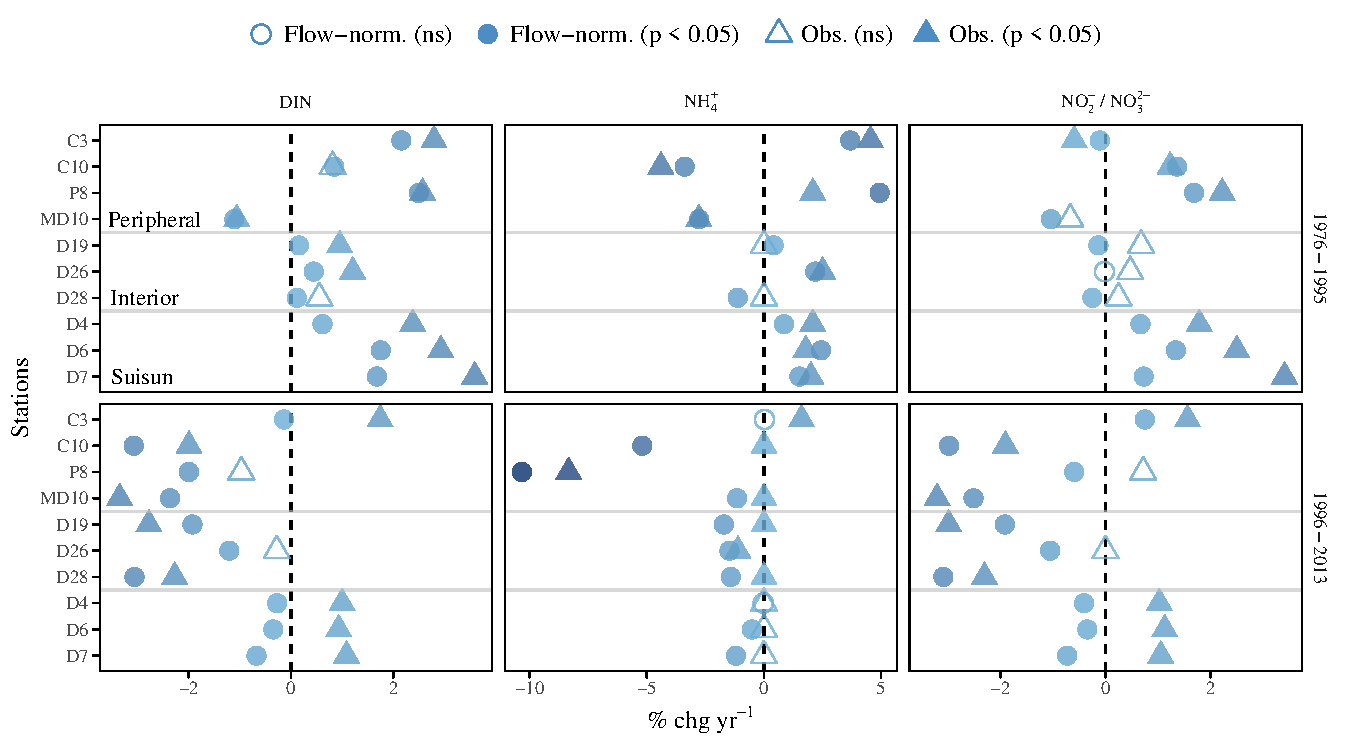
\includegraphics[width = \textwidth]{fig/trndcomp1.pdf}}
\end{frame}

%%%%%%
\begin{frame}{The EPA experience}
\begin{columns}
\begin{column}{0.5\textwidth}
\centerline{
\includegraphics[width=0.3\linewidth]{fig/epa_logo.png}}
\end{column}
\begin{column}{0.5\textwidth}
R-term post-doc, Dec. 2015
\end{column}
\end{columns}
\vspace{0.15in}
\begin{itemize}
\item<+-> You are a federal employee \\~\\
\item<+-> You are not a permanent federal employee \\~\\
\item<+-> You can't tell contractors what to do \\~\\
\item<+-> You can hoard library books
\end{itemize}
\end{frame}

%%%%%%
\begin{frame}{The EPA experience}
\emtxt{4.02B} Nutrient Response and Recovery \\~\\
\begin{itemize}
\item Simulation modelling of NGOM hypoxia  \\~\\
\end{itemize}
\emtxt{4.02A} Microbial Indicators  \\~\\
\begin{itemize}
\item Data munging  \\~\\
\end{itemize}
\emtxt{3.01D} Watershed Sustainability  \\~\\
\begin{itemize}
\item Coral Biocriteria development 
\end{itemize}
\end{frame}

%%%%%%
\begin{frame}{The next chapter}{}

\end{frame}

%%%%%%
\begin{frame}{Final thoughts}{}

\end{frame}

%%%%%%
\begin{frame}{Sincere thank-yous}{}

\end{frame}

%%%%%%
\section{References}
\begin{frame}[allowframebreaks,t]{\textbf{References}}
\tiny
\setbeamertemplate{bibliography item}{}
\bibliographystyle{apalike_mine}
\bibliography{refs}
\end{frame}

\end{document}
